\documentclass[aspectratio=169,10pt]{beamer}

\usetheme{Madrid}
\usecolortheme{seahorse}
\setbeamertemplate{navigation symbols}{}
\setbeamertemplate{footline}[frame number]

\usepackage{amsmath,amssymb,booktabs,array}
\usepackage{tikz}
\usetikzlibrary{arrows.meta,positioning,shapes.geometric,fit,calc}
\usepackage{listings}
\usepackage{xcolor}
\usepackage{hyperref}

\definecolor{codebg}{RGB}{248,248,248}
\definecolor{darkblue}{RGB}{0,65,120}
\definecolor{darkgreen}{RGB}{0,105,70}
\definecolor{warnorange}{RGB}{190,110,0}

\hypersetup{colorlinks=true,linkcolor=darkblue,urlcolor=darkblue}

\lstdefinestyle{shellstyle}{
    basicstyle=\ttfamily\scriptsize,
    keywordstyle=\color{darkblue}\bfseries,
    commentstyle=\color{darkgreen},
    stringstyle=\color{warnorange},
    showstringspaces=false,
    columns=fullflexible,
    backgroundcolor=\color{codebg},
    frame=single,
    rulecolor=\color{black!15},
    breaklines=true
}
\lstset{style=shellstyle}

\newcommand{\code}[1]{\texttt{#1}}
\newcommand{\checkitem}{\textcolor{darkgreen}{\Large$\checkmark$}\;}
\newcommand{\warnitem}{\textcolor{warnorange}{\Large$\triangle$}\;}

\title[Week 1: Kickoff]{Week 1 -- Research Design and Toolchain Kickoff}
\subtitle{Physics-informed AI for Three-phase Unbalanced N-1 Security Screening in Microgrids}
\author{Course Instructor}
\institute{Microgrid 3-phase Security AI Project}
\date{Week 1}

\begin{document}

% ============================================================
\begin{frame}
  \titlepage
  \vspace{-0.8em}
  \begin{center}
    \small Keywords: microgrid, three-phase unbalanced, N-1 screening, physics-informed AI, GNN, pandapower
  \end{center}
\end{frame}

% ============================================================
\begin{frame}{What this lecture covers}
\begin{columns}[T]
\column{0.5\textwidth}
\textbf{Part A -- How this course works}
\begin{itemize}
  \item Textbook learning vs research learning
  \item Working backward from the paper
  \item Mindset shifts you will need
\end{itemize}
\vspace{0.4em}
\textbf{Part B -- Research design}
\begin{itemize}
  \item Why microgrid security is changing
  \item N-1 screening as a research question
  \item Working hypothesis
  \item Eight-week roadmap
\end{itemize}
\column{0.5\textwidth}
\textbf{Part C -- Knowledge stack}
\begin{itemize}
  \item Power systems prerequisites
  \item Machine learning prerequisites
  \item Recommended reading
\end{itemize}
\vspace{0.4em}
\textbf{Part D -- Toolchain setup}
\begin{itemize}
  \item Installing VSCode + micromamba
  \item Creating the \code{pdpower} environment
  \item First notebook smoke test
\end{itemize}
\end{columns}
\vspace{0.5em}
\begin{block}{Goal of Week 1}
By the end of this session, every student should have (a) a clear picture of how this course differs from a typical lecture course, (b) a working development environment, and (c) a mental model of what we are trying to prove over eight weeks.
\end{block}
\end{frame}

% ============================================================
\section*{Part A: How This Course Works}

\begin{frame}{Two modes of learning}
\centering
\scriptsize
\begin{tabular}{p{0.14\textwidth} p{0.37\textwidth} p{0.40\textwidth}}
\toprule
 & \textbf{Textbook learning} & \textbf{Research-style learning} \\
\midrule
Direction & Forward: definitions $\rightarrow$ exercises & Backward: deliverable $\rightarrow$ what we need to learn \\[2pt]
Problems & Closed, a clean answer exists & Open, no oracle anywhere \\[2pt]
Authority & Instructor holds the answer key & No one has the full answer; you become the local expert \\[2pt]
Knowledge & Acquire first, apply later & Acquire because the project needs it now \\[2pt]
Failure & Getting a ``wrong'' answer & A negative result is data, not failure \\[2pt]
Goal & Master a fixed body of material & Produce something that did not exist before \\[2pt]
Assessment & Exam testing recall & Reproducibility, validation, defense of choices \\
\bottomrule
\end{tabular}
\vspace{0.7em}
\normalsize
\begin{block}{Where this course sits}
Most undergrad courses are textbook-mode. This one is research-mode \emph{applied} to a teaching format. The skills it builds --- defining your own question and validating your own work --- are the skills you will need for a thesis and for the first years of a research job.
\end{block}
\end{frame}

% ============================================================
\begin{frame}{Project-driven: working backward from the paper}
The mini-paper at Week 8 is the destination. We work backward to figure out what each earlier week must produce:
\vspace{0.4em}
\centering
\small
\begin{tabular}{rl}
\textbf{Week 8 -- Paper} & needs three model families compared under a screening metric \\
$\downarrow$ & \emph{requires} \\
\textbf{Week 7 -- GNN} & needs a graph dataset and ML baselines to beat \\
$\downarrow$ & \emph{requires} \\
\textbf{Week 6 -- PI-MLP} & needs labeled samples plus a physics-loss design \\
$\downarrow$ & \emph{requires} \\
\textbf{Week 5 -- Baselines} & needs a clean, leakage-free feature table \\
$\downarrow$ & \emph{requires} \\
\textbf{Week 4 -- N-1 labels} & needs many operating scenarios to scan \\
$\downarrow$ & \emph{requires} \\
\textbf{Week 3 -- Scenarios} & needs a working three-phase PF engine \\
$\downarrow$ & \emph{requires} \\
\textbf{Week 2 -- 3-phase PF} & needs an environment and a research question \\
$\downarrow$ & \emph{requires} \\
\textbf{Week 1 -- Today} & alignment on what ``success at Week 8'' means \\
\end{tabular}
\vspace{0.5em}
\normalsize
\begin{block}{Implication for how you study}
Each notebook is a \emph{tool we need to build the next thing}, not a chapter to memorize. If you ever wonder ``why are we doing this?''~--- look one or two weeks ahead.
\end{block}
\end{frame}

% ============================================================
\begin{frame}{Five mindset shifts you will need}
\begin{enumerate}
  \item \textbf{Own your piece.} You will become the local expert on a sub-question nobody else has run before. The instructor is your collaborator, not your answer key.
  \vspace{0.15em}
  \item \textbf{Learn just-in-time, not just-in-case.} Do not read the whole pandapower manual before Week 2. Read the section you need when you need it. The project pulls the knowledge.
  \vspace{0.15em}
  \item \textbf{Validation beats vibes.} ``My code ran'' is not evidence of correctness. Every result needs a proof, a cross-check, or an audit. Roughly 20\% of each week is spent here.
  \vspace{0.15em}
  \item \textbf{Negative results are data.} When the phase-aware GNN underperforms a flat MLP on 77 samples, that is a finding to document, not a failure to hide.
  \vspace{0.15em}
  \item \textbf{``I don't know yet'' is the senior move.} Saying ``I don't know yet, but here is how I will find out'' is more respected than guessing confidently. It is what every working researcher says ten times a day.
\end{enumerate}
\end{frame}

% ============================================================
\section*{Part B: Research Design}

\begin{frame}{Why the grid is harder than ten years ago}
\begin{columns}[T]
\column{0.55\textwidth}
\begin{itemize}
  \item Distributed PV, battery storage, EV charging are now everywhere on the LV side.
  \item Many loads and inverters are \textbf{single-phase}, so the three phases of a feeder no longer carry the same power.
  \item Microgrids can run \emph{grid-connected} or \emph{islanded}; the same fault can have very different consequences.
  \item Operators must decide quickly: \emph{is this state still safe if one component trips?}
\end{itemize}
\column{0.42\textwidth}
\begin{block}{Consequence}
A balanced positive-sequence power flow can declare a feeder safe while one phase is actually undervolt\-age or overloaded. We need phase-aware analysis.
\end{block}
\end{columns}
\end{frame}

% ============================================================
\begin{frame}{Static N-1 security, in one slide}
\begin{columns}[T]
\column{0.5\textwidth}
\begin{block}{N-0 (base case)}
All planned equipment is in service. We check that the power flow converges and that voltages and loadings are inside limits.
\end{block}
\begin{block}{N-1 (contingency)}
Any single critical element trips: a line, a transformer, the PCC tie, a DER, or the battery. We check whether the post-contingency state is still safe.
\end{block}
\column{0.5\textwidth}
\begin{alertblock}{Violation types we will label}
\begin{itemize}
  \item Phase under/over voltage
  \item Line or transformer overload
  \item Voltage unbalance factor (VUF)
  \item Service loss (loads disconnected)
  \item Non-convergence (no feasible solution)
\end{itemize}
\end{alertblock}
\end{columns}
\end{frame}

% ============================================================
\begin{frame}{Why exhaustive N-1 is expensive}
\begin{itemize}
  \item For each operating point $x_t$ and each contingency $c$, we run a three-phase power flow $f_{3\phi}(x_t,c)$.
  \item Realistic studies sweep many scenarios: PV variability, load uncertainty, EV charging, BESS dispatch, daily cycles.
  \item Contingency catalog: line outages, transformer outages, PCC outage, DER trip, BESS trip, switch operations.
  \item Total cost grows as $|\text{scenarios}| \times |\text{contingencies}|$.
\end{itemize}
\begin{block}{Opportunity}
Most contingencies do \emph{not} cause violations. If a fast model can prune the safe ones with high recall, three-phase power flow only needs to be re-run on the suspicious ones.
\end{block}
\end{frame}

% ============================================================
\begin{frame}{The screening idea}
\centering
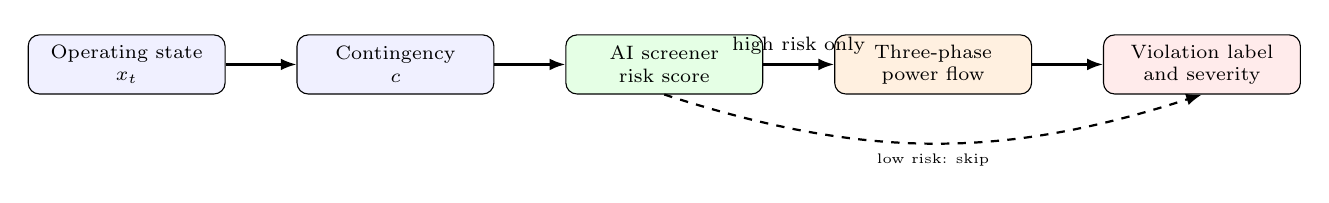
\begin{tikzpicture}[node distance=0.7cm and 0.9cm, every node/.style={font=\scriptsize}]
\tikzset{box/.style={draw, rounded corners, align=center, minimum width=2.5cm, minimum height=0.75cm, fill=blue!6}}
\tikzset{arrow/.style={-{Latex[length=2mm]}, thick}}
\node[box] (state) {Operating state\\$x_t$};
\node[box, right=of state] (cont) {Contingency\\$c$};
\node[box, right=of cont, fill=green!10] (ai) {AI screener\\risk score};
\node[box, right=of ai, fill=orange!12] (pf) {Three-phase\\power flow};
\node[box, right=of pf, fill=red!8] (label) {Violation label\\and severity};
\draw[arrow] (state) -- (cont);
\draw[arrow] (cont) -- (ai);
\draw[arrow] (ai) -- node[above]{high risk only} (pf);
\draw[arrow] (pf) -- (label);
\draw[arrow,dashed] (ai.south) to[bend right=18] node[below,font=\tiny]{low risk: skip} (label.south);
\end{tikzpicture}
\vspace{0.8em}
\begin{block}{Design principle}
The AI model does not replace the power flow. It \emph{prioritizes} which contingencies are worth re-solving. We optimize for \textbf{recall}, not accuracy.
\end{block}
\end{frame}

% ============================================================
\begin{frame}{Research question and hypothesis}
\begin{block}{Research question}
Can a physics-informed, phase-aware AI model maintain very high recall on three-phase N-1 violations while reducing the number of full \code{runpp\_3ph} calls?
\end{block}
\vspace{0.4em}
\begin{block}{Working hypothesis}
If the model jointly uses (i) microgrid topology, (ii) per-phase quantities, (iii) contingency masks, and (iv) physical limit constraints, then it can keep violation recall close to 1.0 while saving 30--60\% of power-flow calls.
\end{block}
\vspace{0.4em}
\begin{alertblock}{What we are \emph{not} claiming}
We are \textbf{not} replacing power-flow software, not solving optimal power flow, and not making deployment-grade claims on a small teaching feeder.
\end{alertblock}
\end{frame}

% ============================================================
\begin{frame}{Eight-week roadmap}
\centering
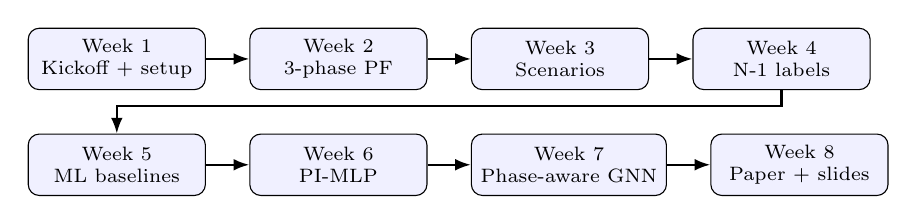
\begin{tikzpicture}[node distance=0.55cm and 0.55cm, every node/.style={font=\scriptsize}]
\tikzset{box/.style={draw, rounded corners, align=center, minimum width=2.25cm, minimum height=0.78cm, fill=blue!6}}
\tikzset{arrow/.style={-{Latex[length=2mm]}, thick}}
\node[box] (w1) {Week 1\\Kickoff + setup};
\node[box, right=of w1] (w2) {Week 2\\3-phase PF};
\node[box, right=of w2] (w3) {Week 3\\Scenarios};
\node[box, right=of w3] (w4) {Week 4\\N-1 labels};
\node[box, below=of w1] (w5) {Week 5\\ML baselines};
\node[box, right=of w5] (w6) {Week 6\\PI-MLP};
\node[box, right=of w6] (w7) {Week 7\\Phase-aware GNN};
\node[box, right=of w7] (w8) {Week 8\\Paper + slides};
\draw[arrow] (w1) -- (w2);
\draw[arrow] (w2) -- (w3);
\draw[arrow] (w3) -- (w4);
\draw[arrow] (w4) -- ++(0,-0.6) -| (w5);
\draw[arrow] (w5) -- (w6);
\draw[arrow] (w6) -- (w7);
\draw[arrow] (w7) -- (w8);
\end{tikzpicture}
\vspace{0.8em}
\begin{block}{Deliverables at the end}
A mini-paper draft (IEEEtran), a 15-slide defense deck, and a validation suite that proves each result.
\end{block}
\end{frame}

% ============================================================
\section*{Part C: Knowledge Stack}

\begin{frame}{What you will need to learn (1/2)}
\begin{columns}[T]
\column{0.5\textwidth}
\textbf{Power systems}
\begin{itemize}
  \item Three-phase circuits, per-unit, $\Delta$/Y connections
  \item Symmetrical components: positive, negative, zero sequence
  \item Voltage unbalance factor (VUF)
  \item AC power flow: Newton-Raphson and backward/forward sweep
  \item Three-phase / asymmetric power flow
  \item N-1 contingency analysis
\end{itemize}
\column{0.5\textwidth}
\textbf{Microgrid engineering}
\begin{itemize}
  \item PCC, DER, BESS, critical load
  \item Grid-connected vs islanded modes
  \item Inverter modeling at a high level
  \item Service-loss and topology connectivity
\end{itemize}
\end{columns}
\vspace{0.5em}
\begin{alertblock}{Honest expectation}
You do not need to be an expert before Week 1. You will learn most of these as we go. But please review three-phase basics and per-unit before Week 2.
\end{alertblock}
\end{frame}

% ============================================================
\begin{frame}{What you will need to learn (2/2)}
\begin{columns}[T]
\column{0.5\textwidth}
\textbf{Machine learning}
\begin{itemize}
  \item Classification, regression, ranking
  \item Train / validation / test splits, group-based CV
  \item Class imbalance, recall, FNR, AUPRC
  \item MLPs and basic PyTorch training loops
  \item Graph Neural Networks (message passing)
  \item Physics-informed loss design
\end{itemize}
\column{0.5\textwidth}
\textbf{Software / engineering}
\begin{itemize}
  \item Python 3, NumPy, pandas, matplotlib
  \item Jupyter notebooks (and how not to abuse them)
  \item VSCode as an IDE
  \item Conda / mamba environments
  \item Reading and using pandapower documentation
\end{itemize}
\end{columns}
\end{frame}

% ============================================================
\begin{frame}{Recommended reading order}
\footnotesize
\begin{enumerate}
  \item \textbf{pandapower documentation} -- start with \emph{Getting Started}, then \emph{AC Power Flow}, then \emph{Asymmetric / Three-phase Power Flow}.
  \item \textbf{Grainger \& Stevenson}, \emph{Power System Analysis} -- chapters on three-phase circuits and symmetrical components.
  \item \textbf{Goodfellow et al.}, \emph{Deep Learning} -- chapter 6 (MLPs) and chapter 7 (regularization).
  \item \textbf{Hamilton}, \emph{Graph Representation Learning} (free online) -- chapters 1--5 cover everything we need for Week 7.
  \item \textbf{Raissi et al.}, \emph{Physics-informed Neural Networks} (JCP 2019) -- the canonical reference for PINN ideas.
\end{enumerate}
\begin{block}{How to use this list}
You are not expected to finish all of these before Week 2. Treat them as a reference you return to when a concept comes up in lecture.
\end{block}
\end{frame}

% ============================================================
\section*{Part D: Toolchain Setup}

\begin{frame}{The setup we are about to do}
\centering
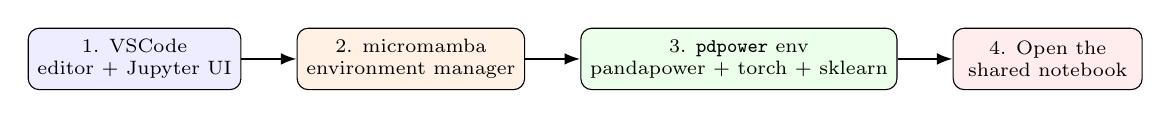
\begin{tikzpicture}[node distance=0.6cm and 0.7cm, every node/.style={font=\scriptsize}]
\tikzset{box/.style={draw, rounded corners, align=center, minimum width=2.4cm, minimum height=0.78cm}}
\tikzset{arrow/.style={-{Latex[length=2mm]}, thick}}
\node[box, fill=blue!7] (vsc) {1. VSCode\\editor + Jupyter UI};
\node[box, fill=orange!10, right=of vsc] (mam) {2. micromamba\\environment manager};
\node[box, fill=green!8, right=of mam] (env) {3. \code{pdpower} env\\pandapower + torch + sklearn};
\node[box, fill=red!7, right=of env] (nb) {4. Open the\\shared notebook};
\draw[arrow] (vsc) -- (mam);
\draw[arrow] (mam) -- (env);
\draw[arrow] (env) -- (nb);
\end{tikzpicture}
\vspace{1em}
\begin{block}{Why this stack}
VSCode + mamba is reproducible across macOS, Linux, and Windows, supports Jupyter inline, and avoids the dependency hell of mixing system Python with pip.
\end{block}
\end{frame}

% ============================================================
\begin{frame}{Step 1: Install VSCode}
\begin{columns}[T]
\column{0.55\textwidth}
\begin{enumerate}
  \item Go to \url{https://code.visualstudio.com/} and download the installer for your OS.
  \item Run the installer with default options.
  \item Launch VSCode and sign in (optional) for settings sync.
  \item Open the Extensions panel (\code{Ctrl+Shift+X} / \code{Cmd+Shift+X}) and install:
  \begin{itemize}
    \item \textbf{Python} (Microsoft)
    \item \textbf{Jupyter} (Microsoft)
    \item \textbf{Pylance} (Microsoft)
  \end{itemize}
\end{enumerate}
\column{0.42\textwidth}
\begin{block}{Why VSCode}
\begin{itemize}
  \item Native Jupyter notebook UI
  \item Same UI on macOS, Linux, and Windows
  \item Strong Python type-checking via Pylance
  \item Lightweight compared to a full IDE
\end{itemize}
\end{block}
\end{columns}
\end{frame}

% ============================================================
\begin{frame}[fragile]{Step 2: Install micromamba (macOS / Linux)}
\textbf{Why micromamba, not Anaconda?}
\begin{itemize}
  \item Single static binary, fast solver (libsolv), no large base environment.
  \item Works exactly the same on macOS, Linux, and inside Docker.
\end{itemize}
\vspace{0.4em}
\textbf{macOS / Linux (recommended one-liner):}
\begin{lstlisting}
"${SHELL}" <(curl -L micro.mamba.pm/install.sh)
\end{lstlisting}
Follow the prompts. The installer adds a \code{micromamba} entry to your shell config (usually \code{\~{}/.zshrc} or \code{\~{}/.bashrc}). Restart the shell after install.
\vspace{0.4em}
\textbf{Verify:}
\begin{lstlisting}
micromamba --version
# 2.x or higher
\end{lstlisting}
\end{frame}

% ============================================================
\begin{frame}[fragile]{Step 2 (alt): Install on Windows}
\textbf{Option A -- Windows PowerShell (native):}
\begin{lstlisting}
Invoke-Expression ((Invoke-WebRequest -Uri https://micro.mamba.pm/install.ps1 -UseBasicParsing).Content)
\end{lstlisting}
\textbf{Option B -- WSL (recommended for this course):}
\begin{enumerate}
  \item Install WSL 2 with Ubuntu from the Microsoft Store.
  \item Open the Ubuntu shell and run the macOS/Linux one-liner from the previous slide.
  \item In VSCode, install the \textbf{WSL} extension. Open notebooks from inside WSL.
\end{enumerate}
\vspace{0.4em}
\begin{alertblock}{Recommendation}
WSL gives a consistent experience with the macOS/Linux instructions used throughout the course. All commands shown later assume a bash/zsh shell.
\end{alertblock}
\end{frame}

% ============================================================
\begin{frame}[fragile]{Step 3: Create the \code{pdpower} environment}
Run the following \emph{one} command in your terminal:
\begin{lstlisting}
micromamba create -n pdpower -c conda-forge -y \
  python=3.11 "pandapower>=3.2" "numpy<2" \
  "pandas<2.3" "scipy<1.14" scikit-learn \
  matplotlib networkx numba pillow pytorch \
  jupyter ipykernel nbconvert
\end{lstlisting}
\vspace{0.3em}
This installs everything we need for the eight weeks:
\begin{itemize}
  \item \code{pandapower>=3.2} -- provides \code{runpp\_3ph} for unbalanced PF.
  \item \code{numpy<2}, \code{pandas<2.3}, \code{scipy<1.14} -- pinned for pandapower compatibility.
  \item \code{pytorch} -- CPU build is fine for this course.
  \item \code{scikit-learn}, \code{matplotlib}, \code{networkx}, \code{numba}, \code{pillow}.
  \item \code{jupyter}, \code{ipykernel}, \code{nbconvert} -- so VSCode can run notebooks.
\end{itemize}
First run downloads $\sim$1.5 GB and takes 5--10 minutes.
\end{frame}

% ============================================================
\begin{frame}[fragile]{Step 4: Activate and verify}
\begin{lstlisting}
micromamba activate pdpower
python --version              # Python 3.11.x
python -c "import pandapower as pp; print(pp.__version__)"
# 3.2.1 or higher
python -c "import torch; print(torch.__version__)"
# 2.x
\end{lstlisting}
\vspace{0.4em}
Quick three-phase power-flow check:
\begin{lstlisting}
python - <<'PY'
import pandapower as pp
from pandapower.networks import ieee_european_lv_asymmetric
net = ieee_european_lv_asymmetric()
pp.runpp_3ph(net)
print("converged:", net.converged, "buses:", len(net.bus))
PY
\end{lstlisting}
You should see \code{converged: True buses: 907}.
\end{frame}

% ============================================================
\begin{frame}[fragile]{Step 5: Open the shared notebook in VSCode}
\begin{enumerate}
  \item Save the \code{.ipynb} file your instructor shared into a folder of your choice.
  \item Open VSCode. Use \code{File $\rightarrow$ Open File...} and select the notebook.
  \item Open the command palette (\code{Cmd/Ctrl+Shift+P}) and run \textbf{Python: Select Interpreter}.
  \item Choose the interpreter under \code{.../envs/pdpower/bin/python}.
  \item Click \textbf{Run All} at the top of the notebook.
\end{enumerate}
\vspace{0.6em}
\begin{block}{Smoke-test pass criteria}
All code cells execute with no error output. If a cell turns red, copy the traceback and bring it to office hours.
\end{block}
\end{frame}

% ============================================================
\begin{frame}[fragile]{Optional: headless smoke test from the terminal}
If you want to verify a notebook without opening VSCode:
\begin{lstlisting}
micromamba run -n pdpower jupyter nbconvert \
  --to notebook --execute path/to/your_notebook.ipynb \
  --output /tmp/smoketest.ipynb \
  --ExecutePreprocessor.timeout=600
\end{lstlisting}
\vspace{0.5em}
Expected output (no traceback):
\begin{lstlisting}
[NbConvertApp] Converting notebook ...
[NbConvertApp] Writing <N> bytes to /tmp/smoketest.ipynb
\end{lstlisting}
If you see this, your environment can execute the course notebooks end-to-end.
\end{frame}

% ============================================================
\begin{frame}{Common pitfalls during setup}
\begin{enumerate}
  \item \warnitem Installing pandapower via \code{pip} on top of system Python. Always create and activate \code{pdpower} first.
  \item \warnitem Using a Python interpreter other than \code{pdpower} in VSCode. Always check the interpreter shown in the bottom-right corner.
  \item \warnitem Installing pandapower 2.x. The course notebooks use 3.x column names (\code{pl\_a\_mw}, \code{ql\_a\_mvar}); 2.x will crash on the first PF result cell.
  \item \warnitem Installing NumPy 2.x. pandapower still imports \code{np.Inf}; pin \code{numpy<2}.
  \item \warnitem Running notebooks on Apple Silicon with a stale x86 conda. Reinstall micromamba native to your CPU.
  \item \warnitem Forgetting to \code{micromamba activate pdpower} before launching Jupyter or running Python.
\end{enumerate}
\end{frame}

% ============================================================
\begin{frame}{Week 1 homework}
\begin{block}{Required}
\begin{enumerate}
  \item Install VSCode, micromamba, and the \code{pdpower} environment on your laptop.
  \item Open the Week 1 notebook your instructor shared and run it end-to-end with zero errors.
  \item Write a 5--8 sentence paragraph: \emph{Why is three-phase unbalanced N-1 screening interesting? What would a successful project look like at the end of Week 8?}
\end{enumerate}
\end{block}
\begin{block}{Optional}
\begin{enumerate}
  \item Open the IEEE European LV asymmetric network in pandapower and plot the bus topology with \code{networkx}.
  \item Run \code{pp.runpp\_3ph(net)} on it and inspect the per-phase voltage distribution.
\end{enumerate}
\end{block}
\end{frame}

% ============================================================
\begin{frame}{Exit checklist}
\begin{enumerate}
  \item \checkitem I can state the research question in one sentence.
  \item \checkitem I can explain why a balanced power flow is insufficient for LV microgrids.
  \item \checkitem I know what \emph{recall}, \emph{FNR}, and \emph{PF calls saved} mean in this project.
  \item \checkitem VSCode is installed with the Python and Jupyter extensions.
  \item \checkitem \code{micromamba --version} works and \code{pdpower} is listed in \code{micromamba env list}.
  \item \checkitem \code{pandapower.runpp\_3ph} converges on the IEEE LV network.
  \item \checkitem I have run the Week 1 notebook end-to-end with no errors.
  \item \checkitem I have a clear mental picture of the eight-week project arc.
\end{enumerate}
\end{frame}

% ============================================================
\begin{frame}{What's next in Week 2}
\begin{columns}[T]
\column{0.55\textwidth}
\textbf{Week 2 will introduce}
\begin{itemize}
  \item \code{create\_asymmetric\_load}, \code{create\_asymmetric\_sgen}
  \item Line zero- and negative-sequence parameters
  \item \code{pp.runpp\_3ph} solver internals
  \item Per-phase result tables: \code{res\_bus\_3ph}, \code{res\_line\_3ph}
  \item Voltage unbalance factor computation
  \item Sanity proofs at $10^{-8}$ tolerance
\end{itemize}
\column{0.42\textwidth}
\begin{alertblock}{Pre-class action}
Make sure your environment passes today's smoke test before Week 2. We will not debug installs during the lecture.
\end{alertblock}
\end{columns}
\end{frame}

% ============================================================
\begin{frame}{References and resources}
\footnotesize
\begin{itemize}
  \item \textbf{pandapower documentation:} \url{https://pandapower.readthedocs.io}
  \item \textbf{micromamba install guide:} \url{https://mamba.readthedocs.io/en/latest/installation/micromamba-installation.html}
  \item \textbf{VSCode Python tutorial:} \url{https://code.visualstudio.com/docs/python/python-tutorial}
  \item \textbf{PyTorch tutorials:} \url{https://pytorch.org/tutorials/}
  \item \textbf{Hamilton, Graph Representation Learning} (free book): \url{https://www.cs.mcgill.ca/~wlh/grl_book/}
  \item \textbf{Raissi, Perdikaris, Karniadakis,} \emph{Physics-informed Neural Networks}, JCP 2019.
\end{itemize}
\vspace{0.8em}
\begin{block}{Office hours}
If you cannot get the environment working after one honest hour of attempts, bring your laptop and the exact error message to office hours. Do not silently struggle for a week.
\end{block}
\end{frame}

\end{document}
